\documentclass[10pt]{iopart}
\usepackage{graphicx}
\usepackage[citestyle=numeric]{biblatex}
\bibliography{B03}
%Uncomment next line if AMS fonts required
%\usepackage{iopams}
\begin{document}


\title[PH1140 Report - T GM Parks]{PH1140 Scientific Skills: Report Poisson statistics using $\gamma$ radiation}

\author{T GM Parks\\28th December 2014}

\begin{abstract}
The distribution of the number of $\gamma$ emissions observed from a radioactive source in a constant time was shown to be modelled by a Poisson distribution. We used a GM tube to count $\gamma$ emissions from a Caesium-137 source for 10 seconds 100 times, and found that all mesurements were within 2\sigma of predicted values.
\end{abstract}

%\maketitle

\section{Introduction}

Raidoactive nuculi are unstable and indidual atoms will decay to states closer to thair ground state, releasing radiation in the process. The liklyhood of any atom or collection of atoms emmitting radiation in a unit time is known to be rrandom and uncorralated. This implies thrugh the the laws of statistics of desicrte events that the sum of events in a time interval will be  Poisson distributed.

The Poisson distribution models the number of discrete events that occur within a time interval, where the events are identical and independent. \cite{mathworld} It is discribed with the mathamatical formula $Poisson(X = x) = \frac{e^{-\gamma }\gamma ^{x}}{x!}$ \cite{riley}

\section{Experimental procedure}

A radioactive source was placed in a Lead cage, 10cm below the aperture for a Geiger-Muller tube. No shielding was placed between the source and the detector, and the experimental apparatus was not changed as data was collected. The GM tube was connected to a timer counter set for a 40kV potential and a 10 second count.
\begin{figure}[htbp]
\begin{center}
\includegraphics[height=5cm]{GMtube.jpg}
\caption{The Geiger-Muller tube connected to the count detector.}
\label{default}
\end{center}
\end{figure}

A 10 second count of radioactive emissions was taken 100 times and recorded. The short integration time for the count was in order to increase the standard deviation of the counts, and make comparison with standard distributions clearer.

A custom Poisson distribution function was created in order to compare the rates at the center of the bins. As the bins were 5 discrete units wide, the center point of the bin was a fractional number (N.5) and so the following implementation of the Poisson distribution was used:

def p(n, mean):
	return ( np.exp(-mean) * mean ** n ) / scipy.misc.factorial(n)

Where the function scipy.misc.factorial implements the Gamma function.

The predicted number of counts for each bin was compared to the Poisson distribution for that bin as shown in \begin{figure}[htbp]
\begin{center}
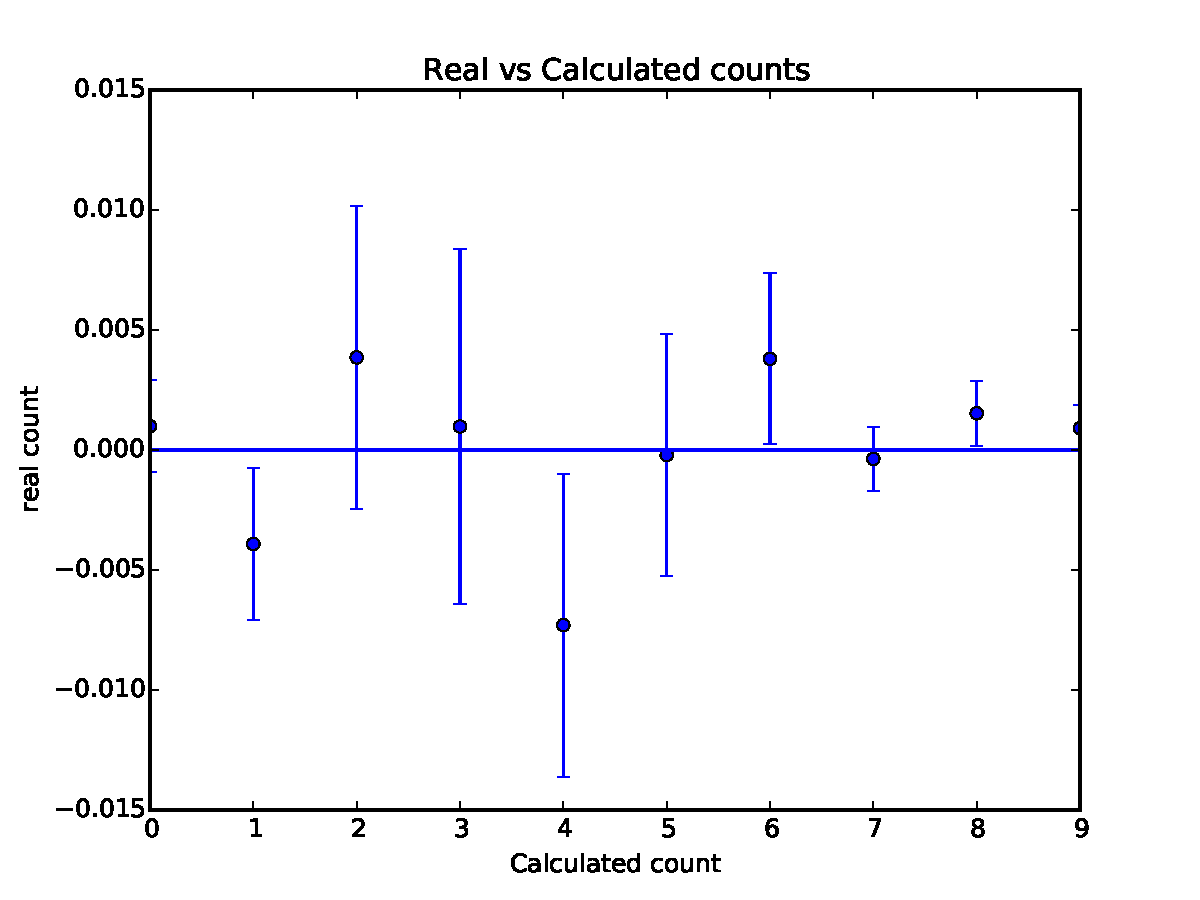
\includegraphics[height=5cm]{errorcomp.pdf}
\caption{default}
\label{default}
\end{center}
\end{figure}
 We found that all the bin counts were within 2 standard deviations, and all but 3 were within a single standard deviation, indicating both a good model fit and good estimation of errors.


\section{Analysis of the data}

\subsection{Comparison with Poisson distribution}

The data was analysed using python and numpy. The mean, standard deviation, and standard error of the mean were calculated
mean:49.161904761904765
standard deviation: 7.549990614341448
error of mean: 0.5222437709993091

    
\section{Summary}

The distribution was found to agree with a Poisson distribution 

\printbibheading
\printbibliography
\end{document}

